% Options for packages loaded elsewhere
\PassOptionsToPackage{unicode}{hyperref}
\PassOptionsToPackage{hyphens}{url}
%
\documentclass[
  8pt,
  ignorenonframetext,
]{beamer}
\usepackage{pgfpages}
\setbeamertemplate{caption}[numbered]
\setbeamertemplate{caption label separator}{: }
\setbeamercolor{caption name}{fg=normal text.fg}
\beamertemplatenavigationsymbolsempty
% Prevent slide breaks in the middle of a paragraph
\widowpenalties 1 10000
\raggedbottom
\setbeamertemplate{part page}{
  \centering
  \begin{beamercolorbox}[sep=16pt,center]{part title}
    \usebeamerfont{part title}\insertpart\par
  \end{beamercolorbox}
}
\setbeamertemplate{section page}{
  \centering
  \begin{beamercolorbox}[sep=12pt,center]{part title}
    \usebeamerfont{section title}\insertsection\par
  \end{beamercolorbox}
}
\setbeamertemplate{subsection page}{
  \centering
  \begin{beamercolorbox}[sep=8pt,center]{part title}
    \usebeamerfont{subsection title}\insertsubsection\par
  \end{beamercolorbox}
}
\AtBeginPart{
  \frame{\partpage}
}
\AtBeginSection{
  \ifbibliography
  \else
    \frame{\sectionpage}
  \fi
}
\AtBeginSubsection{
  \frame{\subsectionpage}
}
\usepackage{amsmath,amssymb}
\usepackage{lmodern}
\usepackage{iftex}
\ifPDFTeX
  \usepackage[T1]{fontenc}
  \usepackage[utf8]{inputenc}
  \usepackage{textcomp} % provide euro and other symbols
\else % if luatex or xetex
  \usepackage{unicode-math}
  \defaultfontfeatures{Scale=MatchLowercase}
  \defaultfontfeatures[\rmfamily]{Ligatures=TeX,Scale=1}
\fi
% Use upquote if available, for straight quotes in verbatim environments
\IfFileExists{upquote.sty}{\usepackage{upquote}}{}
\IfFileExists{microtype.sty}{% use microtype if available
  \usepackage[]{microtype}
  \UseMicrotypeSet[protrusion]{basicmath} % disable protrusion for tt fonts
}{}
\makeatletter
\@ifundefined{KOMAClassName}{% if non-KOMA class
  \IfFileExists{parskip.sty}{%
    \usepackage{parskip}
  }{% else
    \setlength{\parindent}{0pt}
    \setlength{\parskip}{6pt plus 2pt minus 1pt}}
}{% if KOMA class
  \KOMAoptions{parskip=half}}
\makeatother
\usepackage{xcolor}
\newif\ifbibliography
\setlength{\emergencystretch}{3em} % prevent overfull lines
\providecommand{\tightlist}{%
  \setlength{\itemsep}{0pt}\setlength{\parskip}{0pt}}
\setcounter{secnumdepth}{-\maxdimen} % remove section numbering
\newlength{\cslhangindent}
\setlength{\cslhangindent}{1.5em}
\newlength{\csllabelwidth}
\setlength{\csllabelwidth}{3em}
\newlength{\cslentryspacingunit} % times entry-spacing
\setlength{\cslentryspacingunit}{\parskip}
\newenvironment{CSLReferences}[2] % #1 hanging-ident, #2 entry spacing
 {% don't indent paragraphs
  \setlength{\parindent}{0pt}
  % turn on hanging indent if param 1 is 1
  \ifodd #1
  \let\oldpar\par
  \def\par{\hangindent=\cslhangindent\oldpar}
  \fi
  % set entry spacing
  \setlength{\parskip}{#2\cslentryspacingunit}
 }%
 {}
\usepackage{calc}
\newcommand{\CSLBlock}[1]{#1\hfill\break}
\newcommand{\CSLLeftMargin}[1]{\parbox[t]{\csllabelwidth}{#1}}
\newcommand{\CSLRightInline}[1]{\parbox[t]{\linewidth - \csllabelwidth}{#1}\break}
\newcommand{\CSLIndent}[1]{\hspace{\cslhangindent}#1}
% type setting
% ------------------------------------------------------------------------------
\usepackage[german]{babel}     

% fonts
% ------------------------------------------------------------------------------
\usefonttheme{professionalfonts}

% slide title and horizontal line
% ------------------------------------------------------------------------------
\setbeamertemplate{frametitle}{%
    \vskip-30pt \color{black}\large%
    \begin{minipage}[b][23pt]{120mm}%
    \flushleft\insertframetitle%
    \end{minipage}%
}

\setbeamertemplate{headline}										
{
\vskip10pt\hfill\hspace{3.5mm} 										 
\vskip15pt\color{black}\rule{\textwidth}{0.4pt} 					 
}

% slide number
% ---------------------------------------------------------------
\setbeamertemplate{navigation symbols}{}
\setbeamertemplate{footline}
{
\vskip5pt
\vskip2pt
\makebox[123mm]{\hspace{7.5mm}
\hfill Psychologische Forschungsmethoden $\vert$ 
\copyright $ $ 2023 Dirk Ostwald CC BY-SA 4.0 $\vert$ 
Folie \insertframenumber}
\vskip4pt
}

% block color scheme
% ------------------------------------------------------------------------------
% colors
\definecolor{white}{RGB}{255,255,255}
\definecolor{grey}{RGB}{235,235,235}
\definecolor{lightgrey}{RGB}{245,245,245}
\definecolor{LightBlue}{RGB}{220,220,255}
\definecolor{darkblue}{RGB}{51, 51, 153}

% definitions and theorems
\setbeamercolor{block title}{fg = black, bg = grey}
\setbeamercolor{block body}{fg = black, bg = lightgrey}

% general line spacing 
% ------------------------------------------------------------------------------
\linespread{1.3}

% local line spacing
% ------------------------------------------------------------------------------
\usepackage{setspace}

% colors
% -----------------------------------------------------------------------------
\usepackage{color}

% justified text
% ------------------------------------------------------------------------------
\usepackage{ragged2e}
\usepackage{etoolbox}
\apptocmd{\frame}{}{\justifying}{}

% bullet point lists
% -----------------------------------------------------------------------------
\setbeamertemplate{itemize item}[circle]
\setbeamertemplate{itemize subitem}[circle]
\setbeamertemplate{itemize subsubitem}[circle]
\setbeamercolor{itemize item}{fg = black}
\setbeamercolor{itemize subitem}{fg = black}
\setbeamercolor{itemize subsubitem}{fg = black}
\setbeamercolor{enumerate item}{fg = black}
\setbeamercolor{enumerate subitem}{fg = black}
\setbeamercolor{enumerate subsubitem}{fg = black}
\setbeamerfont{itemize/enumerate body}{}
\setbeamerfont{itemize/enumerate subbody}{size = \normalsize}
\setbeamerfont{itemize/enumerate subsubbody}{size = \normalsize}

% color links
% ------------------------------------------------------------------------------
\usepackage{hyperref}
\definecolor{urls}{RGB}{204,0,0}
\hypersetup{colorlinks, citecolor = darkblue, urlcolor = urls}


% additional math commands
% ------------------------------------------------------------------------------
\usepackage{bm}                                         % bold math symbols
\newcommand{\niton}{\not\owns}
\usepackage{cancel}    

% text highlighting
% ------------------------------------------------------------------------------
\usepackage{soul}
\makeatletter
\let\HL\hl
\renewcommand\hl{%
  \let\set@color\beamerorig@set@color
  \let\reset@color\beamerorig@reset@color
  \HL}
\makeatother

% equation highlighting
% -----------------------------------------------------------------------------
\newcommand{\highlight}[2][yellow]{\mathchoice%
  {\colorbox{#1}{$\displaystyle#2$}}%
  {\colorbox{#1}{$\textstyle#2$}}%
  {\colorbox{#1}{$\scriptstyle#2$}}%
  {\colorbox{#1}{$\scriptscriptstyle#2$}}}%

% additional mathematical operators
% ------------------------------------------------------------------------------
\DeclareMathOperator*{\argmax}{arg\,max}
\DeclareMathOperator*{\argmin}{arg\,min}

\ifLuaTeX
  \usepackage{selnolig}  % disable illegal ligatures
\fi
\IfFileExists{bookmark.sty}{\usepackage{bookmark}}{\usepackage{hyperref}}
\IfFileExists{xurl.sty}{\usepackage{xurl}}{} % add URL line breaks if available
\urlstyle{same} % disable monospaced font for URLs
\hypersetup{
  hidelinks,
  pdfcreator={LaTeX via pandoc}}

\author{}
\date{\vspace{-2.5em}}

\begin{document}

\begin{frame}[plain]{}
\protect\hypertarget{section}{}
\center

\begin{center}
\includegraphics[width=0.2\linewidth]{7_Abbildungen/pfm_7_otto} \end{center}

\vspace{2mm}

\Large

Psychologische Forschungsmethoden \vspace{6mm}

\normalsize

BSc Philosophie-Neurowissenschaften-Kognition WiSe 2022/23

BSc Psychologie WiSe 2022/23

\large
\vspace{6mm}

Prof.~Dr.~Dirk Ostwald
\end{frame}

\begin{frame}[plain]{}
\protect\hypertarget{section-1}{}
\vfill
\center
\huge

\textcolor{black}{(7) Skalenarten} \vfill
\end{frame}

\begin{frame}{}
\protect\hypertarget{section-2}{}
\setstretch{1.2}

Überblick \footnotesize

Basierend auf den Beobachtungen zur Bedeutsamkeit von Aussagen bei
Gewichts- und Temperaturmessungen besteht spätestens seit Stevens (1946)
ein Verlangen, zu klassifizieren welche Art von Aussagen und Operationen
im Zahlenraum bei welcher Art von Messproblem angemessen ist.
Traditionell führt dies auf die Begriffe der Ordinal-, Verhältnis, und
Intervallskala, wie in untenstehender Tabelle aus Stevens (1946)
skizziert.

\begin{center}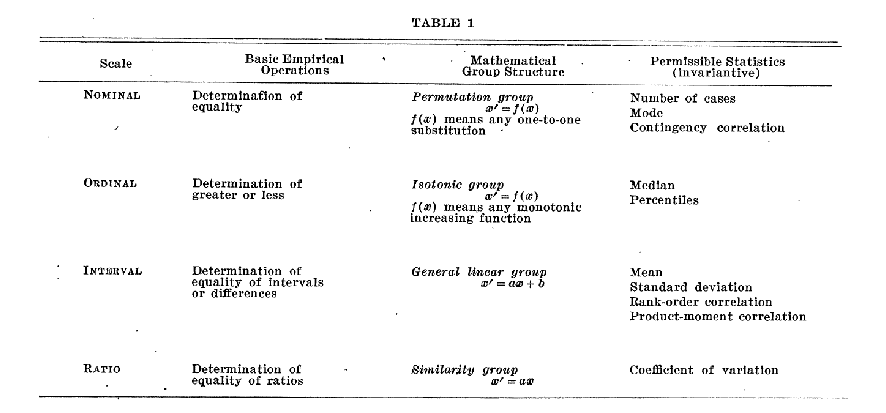
\includegraphics[width=0.7\linewidth]{7_Abbildungen/pfm_7_skalenarten} \end{center}

Die verschiedenen Skalen hier sind im Sinne des Eindeutigkeitsproblems
der Messtheorie eindeutig bis auf eine bestimmte Art von
Funktionstransformation. Es ergibt sich also die Frage, was der Begriff
der ``Skalenart'' bezeichnet und vor dem Hintegrund der Messtheorie
bedeutet. Die folgenden Ausführungen dazu basieren auf Roberts (1984),
Kapitel 2 und insbesondere Roberts and Franke (1976). Die Begriffe der
Ordinal-, Verhältnis-, und Intervallskala stehen in Korrespondenz zu den
Begriffen der Ordinal-, Extensiv-, und Differenzmessung, respektive, die
wir in nachfolgenden Einheiten diskutieren. Den Begriff der Nominalskala
sparen wir aus.
\end{frame}

\begin{frame}{}
\protect\hypertarget{section-3}{}
\vfill
\Large
\setstretch{3.5}

\textbf{Reguläre Repräsentationen}

Skalenarten

Selbstkontrollfragen

\vfill
\end{frame}

\begin{frame}{Reguläre Repräsentationen}
\protect\hypertarget{reguluxe4re-repruxe4sentationen}{}
\footnotesize
\begin{definition}[Zulässige Transformationen einer Skala]
\justifying
Gegeben sei eine Skala $(\mathcal{M},\mathcal{N},f)$ mit zugrundeliegenden Mengen $M$
und $\mathbb{R}$. Sei weiterhin $\phi$ eine Funktion der Form $\phi : f(M) \to \mathbb{R}$, 
wobei $f(M) := \{f(m)|m\in M\}\subseteq \mathbb{R}$ die Bildmenge von $M$ unter $f$ bezeichnet. 
Sei schließlich $\phi \circ f : M \to \mathbb{R}$ die Verkettung von $\phi$ und $f$. 
Dann heißt $\phi$ eine \textit{zulässige Transformation von $(\mathcal{M},\mathcal{N},f)$}, 
wenn $\phi \circ f$ ein Homomorphismus bezüglich $\mathcal{M}$ und $\mathcal{N}$ ist.
\end{definition}
\footnotesize

Bemerkung

\begin{itemize}
\tightlist
\item
  Zur Konstruktion von \(f, \phi\) und \(\phi\circ f\), siehe
  untenstehende Abbildung.
\end{itemize}

\begin{center}\includegraphics[width=0.35\linewidth]{7_Abbildungen/pfm_7_zulässige_skalentransformationen} \end{center}
\end{frame}

\begin{frame}{Reguläre Repräsentationen}
\protect\hypertarget{reguluxe4re-repruxe4sentationen-1}{}
\small

Beispiele

\footnotesize

Es seien \(\mathcal{M} := (\mathbb{N},>)\),
\(\mathcal{N} := (\mathbb{R},>)\) und
\(f : \mathbb{N} \to \mathbb{R}, n \mapsto f(n) := 2n\). Dann ist
\(f \in \mathcal{H}(\mathcal{M},\mathcal{N})\) und
\((\mathcal{M},\mathcal{N},f)\) eine Skala, weil für alle
\(n,m\in \mathbb{N}\) gilt, dass \begin{equation}
n > m \Leftrightarrow 2n > 2m \Leftrightarrow f(n) > f(m).
\end{equation}

\begin{enumerate}
[(1)]
\item
  Es sei nun
  \(\phi : f(\mathbb{N}) \to \mathbb{R}, x \mapsto \phi(x) := x + 5\).
  Dann ist \(\phi\) eine zulässige Transformation von
  \((\mathcal{M},\mathcal{N},f)\), denn auch \begin{equation}
  \phi \circ f : \mathbb{N} \to \mathbb{R}, n \mapsto (\phi \circ f)(n) := \phi(f(n)) = 2n + 5
  \end{equation} ist ein Homomorphismus, weil für alle
  \(n,m\in \mathbb{N}\) auch gilt, dass \begin{equation}
  n > m \Leftrightarrow 2n + 5 > 2m + 5 \Leftrightarrow (\phi \circ f)(n) > (\phi \circ f)(m).
  \end{equation}
\item
  Es sei nun
  \(\phi : f(\mathbb{N}) \to \mathbb{R}, x \mapsto \phi(x) := -x\). Dann
  ist \(\phi\) keine zulässige Transformation von
  \((\mathcal{M},\mathcal{N},f)\), denn \begin{equation}
  \phi \circ f : \mathbb{N} \to \mathbb{R}, n \mapsto (\phi \circ f)(n) := \phi(f(n)) = -2n
  \end{equation} ist kein Homomorphismus, weil für alle
  \(n,m\in \mathbb{N}\) gilt \begin{equation}
  n > m \Leftrightarrow -2n < -2m \,\,\cancel{\Leftrightarrow}\,\, (\phi \circ f)(n) > (\phi \circ f)(m).
  \end{equation}
\end{enumerate}
\end{frame}

\begin{frame}{Reguläre Repräsentationen}
\protect\hypertarget{reguluxe4re-repruxe4sentationen-2}{}
\small
\begin{definition}[Reguläre Skala und reguläre Repräsentation]
\justifying
$\mathcal{M}$ sei ein qualitatives Relationssystem, $\mathcal{N}$ sei ein numerisches
Relationssystem und $\mathcal{H}(\mathcal{M},\mathcal{N})$ sei die Menge der Homomorphismen
von $\mathcal{M}$ nach $\mathcal{N}$. Eine Skala $(\mathcal{M},\mathcal{N},f)$ heißt
\textit{regulär}, wenn zu jedem $g \in \mathcal{H}(\mathcal{M},\mathcal{N})$ eine
Funktion $\phi$ gefunden werden kann, so dass $g = \phi \circ f$ gilt. Wenn jede
Skala $(\mathcal{M},\mathcal{N}, f)$ regulär ist, sagt man, \textit{dass die Repräsentation 
$\mathcal{M}\to \mathcal{N}$ regulär ist}.
\end{definition}

\footnotesize

Bemerkungen

\begin{itemize}
\tightlist
\item
  Reguläre Repräsentationen vereinfachen die Beantwortung des
  Eindeutigkeitsproblems.
\item
  Reguläre Repräsentationen induzieren den Begriff der \emph{Skalenart}.
\item
  Die Regularität einer Repräsentation liegt in der speziellen Form von
  \(\mathcal{M}\) nach \(\mathcal{N}\) begründet.
\end{itemize}
\end{frame}

\begin{frame}{Reguläre Repräsentationen}
\protect\hypertarget{reguluxe4re-repruxe4sentationen-3}{}
\small

\noindent (1) Beispiel für eine reguläre Repräsentation \footnotesize

\footnotesize

Es seien \(\mathcal{M} := (\mathbb{N},>)\),
\(\mathcal{N} := (\mathbb{R},>)\) und \begin{equation}
f : \mathbb{N} \to \mathbb{R}, n \mapsto f(n) := 2n
\end{equation} sowie \begin{equation}
g : \mathbb{N} \to \mathbb{R}, n \mapsto g(n) := 7n
\end{equation} Dann sind
\(f,g\in \mathcal{H}(\mathcal{M}, \mathcal{N})\) und
\((\mathcal{M},\mathcal{N},f)\) und \((\mathcal{M},\mathcal{N},g)\) sind
Skalen. In diesem Fall ergibt sich \begin{equation}
g = \phi \circ f \mbox{ für }\phi : f(M) \to \mathbb{R}, x \mapsto f(x) := \frac{7}{2}x,
\end{equation} denn \begin{equation}
(\phi \circ f)(n) = \phi(2n) = \frac{7}{2}\cdot 2n = 7n = g(n).
\end{equation} Per Konstruktion ist
\(g = \phi\circ f\in \mathcal{H}(\mathcal{M}, \mathcal{N})\) und
\(\phi\) damit eine zulässige Transformation von \(f\).
\end{frame}

\begin{frame}{Reguläre Repräsentationen}
\protect\hypertarget{reguluxe4re-repruxe4sentationen-4}{}
\small
\vspace{1mm}
\setstretch{1.2}

\noindent (2) Beispiel für eine irreguläre Repräsentation \footnotesize

Es sei \(\mathcal{M} := (M,R)\) mit \(M := \{r,s,t\}\) und
\(R := \{(r,s),(r,t)\}\). Weiterhin sei
\(\mathcal{N} := (\mathbb{R},>_{1})\), wobei \begin{equation}
x >_{1} y \Leftrightarrow x > y + 1
\end{equation} für alle \(x,y\in \mathbb{R}\). Dann ist \begin{equation}
f : M \to \mathbb{R} \mbox{ mit } f(r) := 2, f(s) := 0, f(t) := 0
\end{equation} ein Homomorphismus von \(\mathcal{M}\) nach
\(\mathcal{N}\), weil \begin{align}
\begin{split}
(r,s) \in R & \Leftrightarrow 2 > 0 + 1 \Leftrightarrow 2 >_1 0 \Leftrightarrow f(r) >_{1} f(s) \\
(r,t) \in R & \Leftrightarrow 2 > 0 + 1 \Leftrightarrow 2 >_1 0 \Leftrightarrow f(r) >_{1} f(t).
\end{split}
\end{align} Weiterhin ist \begin{equation}
g : M \to \mathbb{R} \mbox{ mit } g(r) := 2.0, g(s) := 0.1, g(t) := 0.0
\end{equation} ein Homomorphismus von \(\mathcal{M}\) nach
\(\mathcal{N}\), weil \begin{align}
\begin{split}
(r,s) \in R & \Leftrightarrow 2.0 > 0.0 + 1 \Leftrightarrow 2 >_1 0.0 \Leftrightarrow g(r) >_{1} g(s) \\
(r,t) \in R & \Leftrightarrow 2.0 > 0.1 + 1 \Leftrightarrow 2 >_1 0.1 \Leftrightarrow g(r) >_{1} g(t).
\end{split}
\end{align} Allerdings existiert keine Funktion der Form
\(\phi:f(M) \to \mathbb{R}\) mit \(g = \phi \circ f\), denn für ein
solches \(\phi\) müsste \begin{equation}
g(s) = (\phi \circ f)(s) = (\phi \circ f)(t) = g(t)
\end{equation} gelten, weil \(f(s) = f(t)\) und \(\phi\) als Funktion
jedem \(x \in f(M)\) genau ein \(\phi(x) \in \mathbb{R}\) zuordnet.

Es gilt aber nach Definition \(g(s) = 0.1 \neq 0.0 = g(t)\).
\end{frame}

\begin{frame}{Reguläre Repräsentationen}
\protect\hypertarget{reguluxe4re-repruxe4sentationen-5}{}
\small
\vspace{1mm}
\setstretch{1.2}
\begin{theorem}[Charakterisierung regulärer Skalen]
\justifying
\normalfont
Eine Skala $(\mathcal{M}, \mathcal{N},f)$ ist dann und nur dann regulär, wenn
für alle $g \in \mathcal{H}(\mathcal{M}, \mathcal{N})$ und $m,n \in M$ gilt, dass
aus $f(m) = f(n)$ folgt, dass $g(m) = g(n)$.
\end{theorem}

\footnotesize

\underline{Beweis}

\emph{Beweis von ``\((\mathcal{M}, \mathcal{N},f)\) ist regulär
\(\Rightarrow\) Aus \(f(m) = f(n)\) folgt, dass \(g(m) = g(n)\).''}

Sei zunächst \((\mathcal{M}, \mathcal{N},f)\) ein reguläre Skala. Dann
existiert für jede beliebige Skala \((\mathcal{M}, \mathcal{N},g)\),
also insbesondere für jedes
\(g \in \mathcal{H}(\mathcal{M}, \mathcal{N})\) eine Funktion der Form
\(\phi : f(M) \to \mathbb{R}\), so dass \(g = \phi \circ f\). Es gilt
also \begin{equation}
f(m) = f(n) \Rightarrow (\phi \circ f)(m) = (\phi \circ f)(n) \Leftrightarrow g(m) = g(n),
\end{equation} da \(\phi\) als Funktion jedem \(x \in f(M)\) genau ein
(und nicht etwa mehrere) \(\phi(x)\) zuordnet.

\vspace{1mm}

\emph{Beweis von ``Aus \(f(m) = f(n)\) folgt, dass
\(g(m) = g(n) \Rightarrow (\mathcal{M}, \mathcal{N},f)\) ist regulär.''}

Sei umgekehrt ein \(g \in \mathcal{H}(\mathcal{M}, \mathcal{N})\) mit
\(g(m) = g(n)\) und definiere \begin{equation}
\phi \circ f : f(M) \to \mathbb{R}, m \mapsto (\phi \circ f)(m) := g(m).
\end{equation} Dann gilt, weil aus \(f(m) = f(n)\) folgt, dass
\(g(m) = g(n)\) und damit \((\phi \circ f)(m) := (\phi \circ f)(n)\)
ist, dass \(\phi\) eine Funktion ist, also jedem \(x \in f(M)\) genau
ein (und nicht etwa mehrere) \(\phi(x)\) zuordnet. Weiterhin ist
\(g = \phi \circ f\). Es existiert also für eine beliebige Skala
\((\mathcal{M}, \mathcal{N},g)\) eine Funktion der Form
\(\phi \circ f : f(M) \to \mathbb{R}\) mit \(g = \phi \circ f\), und
damit ist die Skala \((\mathcal{M}, \mathcal{N},f)\) regulär.

\(\hfill\Box\)
\end{frame}

\begin{frame}{Reguläre Repräsentationen}
\protect\hypertarget{reguluxe4re-repruxe4sentationen-6}{}
\small
\begin{theorem}[Isomorphismen und Regulärität]
\justifying
\normalfont
Wenn $f$ ein Isomorphismus ist, dann ist $(\mathcal{M}, \mathcal{N},f)$ regulär.
\end{theorem}

\footnotesize

\underline{Beweis}

Wenn \(f\) ein Isomorphismus ist, dann ist \(f\) ein injektiver
Homomorphismus von \(\mathcal{M}\) nach \(\mathcal{N}\). Insbesondere
gilt für \(f\) also, dass aus \(f(m) = f(n)\) folgt, dass \(m = n\) ist.
Sei \(g\) ein weiterer Homomorphismus von \(\mathcal{M}\) nach
\(\mathcal{N}\). Dann ist \(g\) insbesondere eine Abbildung von \(M\)
nach \(\mathbb{R}\) und ordnet jedem \(m \in M\) genau ein
\(g(m) \in \mathbb{R}\) zu. Also folgt aus \(m = n\), dass
\(g(m) = g(n)\). Also impliziert für einen Isomorphismus und alle
\(m,n \in M\) \(f(m) = f(n)\) immer, dass für einen weiteren
Homomorphismus \(g\) von \(\mathcal{M}\) nach \(\mathcal{N}\) gilt, dass
\(g(m) = g(n)\) und dies ist gerade die Bedingung für die Regularität
von \((\mathcal{M}, \mathcal{N},f)\) nach dem Theorem zur
Charakterisierung regulärer Skalen.

\(\hfill\Box\)
\end{frame}

\begin{frame}{}
\protect\hypertarget{section-4}{}
\vfill
\Large
\setstretch{3.5}

Reguläre Skalen

\textbf{Skalenarten}

Selbstkontrollfragen \vfill
\end{frame}

\begin{frame}{Skalenarten}
\protect\hypertarget{skalenarten}{}
\footnotesize
\begin{definition}[Skalenart]
\justifying
Gegeben sei eine Skala $(\mathcal{M},\mathcal{N},f)$ mit zugrundeliegenden Mengen
$M$ und $\mathbb{R}$ und Homomorphismus $f$. Weiterhin sei 
\begin{equation}
\Phi := \{\phi| \phi : f(M) \to \mathbb{R} \}
\end{equation}
eine \textit{Klasse von Funktionen}. Wenn $\Phi$ die Menge der zulässigen Transformationen 
der Skala $(\mathcal{M},\mathcal{N},f)$ ist, dann sagt man, dass  $(\mathcal{M},\mathcal{N},f)$ 
von gleicher Skalenart sind.
\end{definition}

Bemerkungen

\begin{itemize}
\item Primär von Interesse sind im Folgenden folgende Funktionenklassen
\begin{itemize}
\begin{footnotesize}
\item Die Klasse der \textit{monoton steigenden Funktionen}
\begin{equation}
\Phi := \{\phi| \phi : f(M) \to \mathbb{R}, x \mapsto \phi(x)  \mbox{ mit } x > y \Leftrightarrow f(x) > f(y) \mbox{ für alle } x,y \in f(M)\}
\end{equation}
\item Die Klasse der \textit{Ähnlichkeitstransformationen}
\begin{equation}
\Phi := \{\phi| \phi : f(M) \to \mathbb{R}, x \mapsto \phi(x) := \alpha x \mbox{ mit } \alpha > 0\}
\end{equation}
\item Die Klasse der \textit{positiv linear-affinen Transformationen}
\begin{equation}
\Phi := \{\phi| \phi : f(M) \to \mathbb{R}, x \mapsto \phi(x) := \alpha x + \beta  \mbox{ mit } \alpha > 0\}
\end{equation}
\end{footnotesize}
\end{itemize}
\end{itemize}
\end{frame}

\begin{frame}{Skalenarten}
\protect\hypertarget{skalenarten-1}{}
\footnotesize
\begin{definition}[Ordinalskala]
\justifying
Gegeben sei eine Skala $(\mathcal{M},\mathcal{N},f)$ mit zugrundeliegenden Mengen
$M$ und $\mathbb{R}$. Wenn die Klasse der zulässigen Transformationen von 
$(\mathcal{M},\mathcal{N},f)$ die Klasse der \textit{monoton steigenden Funktionen} 
\begin{equation}
\Phi := \{\phi| \phi : f(M) \to \mathbb{R}, x \mapsto \phi(x)  \mbox{ mit } x > y \Leftrightarrow f(x) > f(y) \mbox{ für alle } x,y \in f(M)\}
\end{equation}
ist, dann heißt $(\mathcal{M},\mathcal{N},f)$ \textit{Ordinalskala}.
\end{definition}

Bemerkungen

\begin{itemize}
\tightlist
\item
  Wir werden in Einheit (9) sehen, dass Ordinalmessungen Ordinalskalen
  induzieren.
\item
  Ein prototypische Beispiel für Ordinalmessungen ist das Messen von
  Entscheidungsoptionspräferenzen.
\end{itemize}
\end{frame}

\begin{frame}{Skalenarten}
\protect\hypertarget{skalenarten-2}{}
\footnotesize
\begin{definition}[Verhältnisskala]
\justifying
Gegeben sei eine Skala $(\mathcal{M},\mathcal{N},f)$ mit zugrundeliegenen Mengen
$M$ und $\mathbb{R}$ und Homomorphismus $f$. Wenn die Klasse der zulässigen
Transformationen der Skala $(\mathcal{M},\mathcal{N},f)$ die Klasse der 
\textit{Ähnlichkeitstransformationen}
\begin{equation}
\Phi := \{\phi| \phi : f(M) \to \mathbb{R}, x \mapsto \phi(x) := \alpha x \mbox{ mit } \alpha > 0\}
\end{equation}
ist, dann heißt $(\mathcal{M},\mathcal{N},f)$ \textit{Verhältnisskala}.
\end{definition}

Bemerkungen

\begin{itemize}
\tightlist
\item
  Wir werden in Einheit (9) sehen, dass Extensivmessungen
  Verhältnisskalen induzieren.
\item
  Das prototypische Beispiel für eine Extensivmessung ist das Messen des
  Gewichts eines Objekts.
\end{itemize}
\end{frame}

\begin{frame}{Skalenarten}
\protect\hypertarget{skalenarten-3}{}
\footnotesize
\begin{definition}[Intervallskala]
\justifying
Gegeben sei eine Skala $(\mathcal{M},\mathcal{N},f)$ mit zugrundeliegenen Mengen
$M$ und $\mathbb{R}$ und Homomorphismus $f$. Wenn die Klasse der zulässigen
Transformationen der Skala $(\mathcal{M},\mathcal{N},f)$ die Klasse der 
\textit{positiv linear-affinen Transformationen}
\begin{equation}
\Phi := \{\phi| \phi : f(M) \to \mathbb{R}, x \mapsto \phi(x) := \alpha x + \beta  \mbox{ mit } \alpha > 0\}
\end{equation}
ist, dann heißt $(\mathcal{M},\mathcal{N},f)$ \textit{Intervallskala}.
\end{definition}

Bemerkungen

\begin{itemize}
\tightlist
\item
  Wir werden in Einheit (11) sehen, dass Differenzmessungen
  Intervallskalen induzieren.
\item
  Das prototypische Beispiel für Differenzmessungen ist das Messen der
  Temperatur in Celsius oder Fahrenheit.
\end{itemize}
\end{frame}

\begin{frame}{Skalenarten}
\protect\hypertarget{skalenarten-4}{}
\vspace{1mm}
\small

Beispiel (1) Nachweis der Ordinalskalenart einer Skala

\footnotesize
\setstretch{1.2}

Gegeben sei das qualitative Relationssystem \(\mathcal{M} := (M,R)\) mit
\begin{equation}
M := \{r,s,t\} \mbox{ und } R := \{(r,s),(s,t),(r,t)\}
\end{equation} \(\mathcal{M}\) ist homomorph zu dem numerischen
Relationssystem \(\mathcal{N} := (\mathbb{R},>)\), denn mit
\begin{equation}
f : M \to \mathbb{R} \mbox{ mit } f(r) := 2, f(s) := 1, f(t) = 0
\end{equation} existiert ein Homomorphismus von \(\mathcal{M}\) nach
\(\mathcal{N}\) und
\(\mathcal{H}(\mathcal{M},\mathcal{N})\neq \emptyset\): \begin{align}
\begin{split}
(r,s) \in R & \Leftrightarrow 2 > 1 \Leftrightarrow f(r) > f(s) \Leftrightarrow (f(r), f(s)) \in\, > \\
(s,t) \in R & \Leftrightarrow 1 > 0 \Leftrightarrow f(s) > f(t) \Leftrightarrow (f(s), f(t)) \in\, > \\
(r,t) \in R & \Leftrightarrow 2 > 0 \Leftrightarrow f(r) > f(t) \Leftrightarrow (f(r), f(t)) \in\, > \\
\end{split}
\end{align} Da \(f\) weiterhin injektiv ist, ist die Repräsentation
regulär. Weiterhin ist \(\phi\) eine zulässige Transformation von \(f\)
dann und nur dann, wenn \(g := \phi \circ f\) wiederum ein
Homomorphismus von \(\mathcal{M}\) nach \(\mathcal{N}\) ist, wenn also
gilt \begin{align}
\begin{split}
g(r) > g(s) & \Leftrightarrow (\phi \circ f)(r) > (\phi \circ f)(s) \Leftrightarrow \phi(2) > \phi(1) \\
g(s) > g(t) & \Leftrightarrow (\phi \circ f)(s) > (\phi \circ f)(t) \Leftrightarrow \phi(1) > \phi(0) \\
g(r) > g(t) & \Leftrightarrow (\phi \circ f)(r) > (\phi \circ f)(t) \Leftrightarrow \phi(2) > \phi(0) \\
\end{split}
\end{align} Dann gilt für \(\phi\) mit \(f(M) := \{0,1,2\}\) aber, dass
\begin{equation}
\phi : f(M) \to \mathbb{R}, x \mapsto \phi(x)  \mbox{ mit } x > y \Leftrightarrow f(x) > f(y) \mbox{ für alle } x,y \in f(M)
\end{equation} und \(\phi\) ist dann und nur dann eine zulässige
Transformation von \(f\), wenn \(\phi\) eine monoton steigende Funktion
ist. Damit ist \((\mathcal{M}, \mathcal{N},f)\) eine Ordinalskala.
\end{frame}

\begin{frame}{Skalenarten}
\protect\hypertarget{skalenarten-5}{}
\small
\begin{theorem}[Skalenart]
\justifying
\normalfont
Wenn eine Repräsentation $\mathcal{M} \to  \mathcal{N}$ regulär ist und wenn
$f$ und $g$ Homormorphismen von $\mathcal{M}$ nach $\mathcal{N}$ sind, dann ist 
$f$ eine Ordinalskala, Verhältnisskala, oder Intervallskala genau dann und nur 
dann, wenn $g$ eine Ordinalskala, Verhältnisskala, oder Intervallskala, respektive, ist.
\end{theorem}
\footnotesize

Bemerkungen

\begin{itemize}
\tightlist
\item
  Bei regulären Repräsentationen sind also alle Skalen von der gleichen
  Skalenart.
\item
  Die Regularität einer Repräsentation liegt in der speziellen Form von
  \(\mathcal{M}\) nach \(\mathcal{N}\) begründet.
\item
  Im Folgenden betrachten wir, wie \(\mathcal{M}\) und \(\mathcal{N}\)
  beschaffen sein müssen, um obige Skalenarten zu induzieren.
\end{itemize}
\end{frame}

\begin{frame}{Skalenarten}
\protect\hypertarget{skalenarten-6}{}
\footnotesize

\underline{Beweis}

Wir beweisen das Theorem nur für den Fall einer Ordinalskala. Wir zeigen
dabei auch lediglich, dass aus der Regularität von
\(\mathcal{M} \to \mathcal{N}\) und der Tatsache, dass \(f\) eine
Ordinalskala ist, folgt, dass ein weiterer Homomorphismus \(g\) von
\(\mathcal{M}\) nach \(\mathcal{N}\) ebenfalls eine Ordinalskala ist.

\(f\) sei eine Ordinalskala. Wir halten zunächst fest, dass weil die
Repräsentation \(\mathcal{M} \to \mathcal{N}\) regulär ist, es ein
\(\phi : f(M) \to \mathbb{R}\) mit \(g = \phi \circ f\) gibt. Weiterhin
gilt, dass weil \(g\) ein Homomorphismus ist, ein solches \(\phi\) eine
zulässige Transformation von \(f\) ist. Schließlich gilt, dass weil
\(f\) eine Ordinalskala ist und damit per Definition alle zulässigen
Transformationen von \(f\) monoton steigende Funktionen sind, ein
solches \(\phi\) eine monoton steigende Funktion ist.

Der restliche Beweis erfolgt durch Beweis folgender Implikationen:

\begin{enumerate}
[(1)]
\tightlist
\item
  \(\phi' : g(M) \to \mathbb{R}\) ist monoton steigend
  \(\quad\,\,\Rightarrow\) \(\phi'\) ist eine zulässige Transformation
  von \(g\).
\item
  \(\phi'\) ist eine zulässige Transformation von
  \(g \Rightarrow \phi' : g(M) \to \mathbb{R}\) ist monoton steigend.
\end{enumerate}

Also gilt \begin{equation}
\phi' \mbox{ ist eine zulässige Transformation von } g \Leftrightarrow \phi' : g(M) \to \mathbb{R} \mbox{ ist monoton steigend}.
\end{equation} Die Klasse der zulässigen Transformation von \(g\) ist
damit also die Klasse der monoton steigenden Funktionen und \(g\) ist
damit eine Ordinalskala.
\end{frame}

\begin{frame}{Skalenarten}
\protect\hypertarget{skalenarten-7}{}
\footnotesize

\underline{Beweis}

\emph{Beweis der Implikation (1) \(\phi' : g(M) \to \mathbb{R}\) ist
monoton steigend \(\Rightarrow\) \(\phi'\) ist eine zulässige
Transformation von \(g\)}

Die Implikation gilt, weil mit obigem \(\phi\) gilt, dass
\begin{equation}
\phi' \circ g = \phi' \circ (\phi \circ f) = (\phi' \circ \phi) \circ f.
\end{equation} Weil \(\phi'\) und \(\phi\) monoton steigende Funktionen
sind, ist \(\phi' \circ \phi\) auch monoton steigend und damit eine
zulässige Transformation von \(f\). Damit ist wiederum \(\phi'\circ g\)
ein Homomorphismus von \(\mathcal{M}\) nach \(\mathcal{N}\) und
\(\phi'\) daher eine zulässige Transformation von \(g\). \vspace{1mm}

\emph{Beweis der Implikation (2) \(\phi'\) ist eine zulässige
Transformation von \(g \Rightarrow \phi' : g(M) \to \mathbb{R}\) ist
monoton steigend}

Die Implikation gilt, weil mit obigem \(\phi\) gilt, dass
\begin{equation}
\phi' \circ g = \phi' \circ (\phi \circ f) = (\phi' \circ \phi) \circ f
\end{equation} ein Homorphismus von \(\mathcal{M}\) nach \(\mathcal{N}\)
ist und \(\phi' \circ \phi\) somit eine zulässige Transformation \(f\).
Damit muss \(\phi' \circ \phi\) aber eine monoton steigende Funktion
sein und deshalb auch \(\phi'\).
\end{frame}

\begin{frame}{Skalenarten}
\protect\hypertarget{skalenarten-8}{}
\setstretch{2}
\small

Weitere Skalenarten

\footnotesize

Man unterscheidet weiterhin mindestens folgende Skalenarten:

\center
\begin{tabular}{ll}
Name                & Menge der zulässigen Transformationen                                                                     \\\hline
Absolutskala        & $\Phi := \{\phi| \phi : f(M) \to \mathbb{R}, x \mapsto \phi(x) := x\}$                                    \\
Log-Intervallskala  & $\Phi := \{\phi| \phi : f(M) \to \mathbb{R}, x \mapsto \phi(x) := \alpha x^{\beta}, \alpha,\beta >0\}$    \\
Differenzskala      & $\Phi := \{\phi| \phi : f(M) \to \mathbb{R}, x \mapsto \phi(x) := x - \beta, \beta \in \mathbb{R}\}$      \\
Nominalskala        & $\Phi := \{\phi| \phi : f(M) \to \mathbb{R} \mbox{ und } \phi \mbox{ ist injektiv}\}$                     \\\hline
\end{tabular}

\begin{itemize}
\tightlist
\item
  Jede dieser Skalenarten ist durch die spezielle Form von
  \(\mathcal{M}\) und \(\mathcal{N}\) determiniert.
\item
  Im Rahmen dieser Einführung verzichten wir auf eine detaillierte
  Diskussion ihrer Repräsentationen.
\item
  Log-Intervallskalen werden uns jedoch in Einheit (12) Psychophysik
  begegnen.
\end{itemize}
\end{frame}

\begin{frame}{}
\protect\hypertarget{section-5}{}
\vfill
\Large
\setstretch{3.5}

Reguläre Skalen

Skalenarten

\textbf{Selbstkontrollfragen} \vfill
\end{frame}

\begin{frame}{Selbstkontrollfragen}
\protect\hypertarget{selbstkontrollfragen}{}
\small
\setstretch{3}

\begin{enumerate}
\tightlist
\item
  Definieren Sie den Begriff der zulässigen Transformation einer Skala.
\item
  Definieren Sie die Begriffe der regulären Skala und der regulären
  Repräsentation.
\item
  Definieren Sie den Begriff der Skalenart.
\item
  Definieren Sie den Begriff der Ordinalskala.
\item
  Definieren Sie den Begriff der Verhältnisskala.
\item
  Definieren Sie den Begriff der Intervallskala.
\item
  Geben Sie das Theorem zur Skalenart wieder.
\end{enumerate}
\end{frame}

\begin{frame}{Referenzen}
\protect\hypertarget{referenzen}{}
\footnotesize

\hypertarget{refs}{}
\begin{CSLReferences}{1}{0}
\leavevmode\vadjust pre{\hypertarget{ref-roberts_1984}{}}%
Roberts, Fred S. 1984. \emph{Measurement Theory with Applications to
Decisionmaking, Utility, and the Social Sciences}. Encyclopedia of
Mathematics and Its Applications ; {Section}, {Mathematics} and the
Social Sciences, v. 7. Cambridge {[}Cambridgeshire{]} ; New York, NY,
USA: Cambridge University Press.

\leavevmode\vadjust pre{\hypertarget{ref-roberts_1976}{}}%
Roberts, Fred S., and Charles H. Franke. 1976. {``On the Theory of
Uniqueness in Measurement.''} \emph{Journal of Mathematical Psychology}
14 (3): 211--18. \url{https://doi.org/10.1016/0022-2496(76)90002-X}.

\leavevmode\vadjust pre{\hypertarget{ref-stevens_1946}{}}%
Stevens, S. S. 1946. {``On the {Theory} of {Scales} of {Measurement}.''}
\emph{Science, New Series} 103 (2684): 677--80.
\url{http://www.jstor.org/stable/1671815}.

\end{CSLReferences}
\end{frame}

\end{document}
